% !TEX program = xelatex
% 딥러닝분석 파이널 프로젝트 보고서 — 한국어(fontspec + Noto CJK)
\documentclass[11pt]{article}

\usepackage{fontspec}
% 한글 폰트 폴백 체인: 서버에 무엇이 있든 PDF가 나오도록 (XeLaTeX 필수)
\IfFontExistsTF{Noto Serif CJK KR}{\setmainfont{Noto Serif CJK KR}[AutoFakeSlant=0.18]}{%
 \IfFontExistsTF{Noto Serif KR}{\setmainfont{Noto Serif KR}[AutoFakeSlant=0.18]}{%
  \IfFontExistsTF{UnBatang}{\setmainfont{UnBatang}[AutoFakeSlant=0.18]}{%
   \IfFontExistsTF{NanumMyeongjo}{\setmainfont{NanumMyeongjo}[AutoFakeSlant=0.18]}{}}}}
\IfFontExistsTF{Noto Sans CJK KR}{\setsansfont{Noto Sans CJK KR}[AutoFakeSlant=0.18]}{%
 \IfFontExistsTF{Noto Sans KR}{\setsansfont{Noto Sans KR}[AutoFakeSlant=0.18]}{%
  \IfFontExistsTF{UnDotum}{\setsansfont{UnDotum}}{%
   \IfFontExistsTF{NanumGothic}{\setsansfont{NanumGothic}}{}}}}
\IfFontExistsTF{Noto Sans Mono CJK KR}{\setmonofont{Noto Sans Mono CJK KR}}{%
 \IfFontExistsTF{UnDotum}{\setmonofont{UnDotum}}{%
  \IfFontExistsTF{NanumGothicCoding}{\setmonofont{NanumGothicCoding}}{}}}
\XeTeXlinebreaklocale "ko"
\XeTeXlinebreakskip = 0pt plus 0.1pt

\usepackage[a4paper,top=22mm,bottom=22mm,left=27mm,right=27mm]{geometry}
\usepackage{graphicx}
\usepackage{booktabs}
\usepackage{array}
\usepackage{amsmath}
\usepackage{amssymb}
\usepackage{xcolor}
\usepackage{caption}
\usepackage{subcaption}
\usepackage{enumitem}
\usepackage{titlesec}
\usepackage{fancyhdr}
\usepackage{float}
\usepackage{etoolbox}
\usepackage{setspace}
\setstretch{1.28}
\usepackage[colorlinks=true,linkcolor=black,citecolor=black,urlcolor=blue!60!black]{hyperref}

% 표는 본문보다 한 단계 작게 + 행간 보통으로 (가독성·폭 안정)
\AtBeginEnvironment{table}{\small\setstretch{1.0}}

% ── 스타일 (정통 논문 룩: 흑백·세리프) ───────────────────────────────────────
\captionsetup{font=small,labelfont=bf,skip=4pt}
\captionsetup[figure]{name=그림}
\captionsetup[table]{name=표}
\renewcommand{\figurename}{그림}
\renewcommand{\tablename}{표}
\setlist{leftmargin=1.5em,itemsep=2pt,topsep=3pt,parsep=0pt}
\setlength{\tabcolsep}{5pt}

\titleformat{\section}{\large\bfseries}{\thesection}{0.6em}{}
\titleformat{\subsection}{\normalsize\bfseries}{\thesubsection}{0.5em}{}
\titlespacing{\section}{0pt}{8pt}{3pt}
\titlespacing{\subsection}{0pt}{6pt}{2pt}

\pagestyle{plain}

\setlength{\parindent}{0pt}
\setlength{\parskip}{3pt}
\renewcommand{\arraystretch}{1.1}

% 초록 블록 (양쪽 들여쓰기 + 작은 글씨)
\newenvironment{abstractblock}{%
  \begin{center}\textbf{초록}\end{center}\vspace{-4pt}%
  \begin{list}{}{\setlength{\leftmargin}{1.6em}\setlength{\rightmargin}{1.6em}}\item[]\small}%
  {\end{list}\vspace{2pt}}

\begin{document}

% ── 기본 정보 ────────────────────────────────────────────────────────────────
\begin{center}
{\LARGE\bfseries 한국어 주식 댓글의 주가 예측 적중 분류}\\[5pt]
{\large 댓글 텍스트만으로 적중한 예측을 식별할 수 있는가}\\[10pt]
{\normalsize 남\,채\,린}\\[3pt]
{\footnotesize 숭실대학교 AI소프트웨어학부 · 딥러닝분석 · 2분반 18조 · 학번 20223074}
\end{center}
\vspace{6pt}

\begin{abstractblock}
본 보고서는 \emph{주가를 적중시킨 예측 댓글을 댓글 텍스트만으로 식별할 수 있는가}라는 문제를 다룬다. 이를 위해 종목 댓글을 예측 적중 정도에 따라 네 가지 클래스(예측 없음, 예측 실패, 방향 적중, 날짜·방향 적중)로 정의하고, 미래 주가를 입력에서 배제한 누수 없는 자동 라벨링 파이프라인을 구축하였다. 라벨링된 데이터로 한국어 사전학습 인코더를 미세조정하여 적중 댓글 식별 분류기를 학습하고, 종목을 분리한 교차 평가로 일반화를 검증하였다. 최우수 모델의 macro-F1은 0.389로, 기준선인 다수 클래스 0.231과 TF-IDF 0.323보다 높았다. 텍스트만으로도 적중 댓글을 어느 정도 가려낼 수 있다는 뜻이다. 다만 적중에 해당하는 소수 클래스의 성능은 낮으며, 작성자 단위 보조 분석에서도 꾸준히 적중하는 작성자가 있는 듯 보였으나 전·후반으로 나누면 그 경향이 유지되지 않았다. 본 보고서는 적중 식별이 가능한 수준과 그 한계를 정량적으로 제시하고, 그 한계가 신호의 부재가 아니라 적중 표본의 희소성에서 비롯됨을 밝힌다.
\end{abstractblock}

% ── 1. 서론 ─────────────────────────────────────────────────────────────────
\section{서론}

종목 토론 댓글에는 주가를 적중시킨 예측이 섞여 있다. 이러한 적중 댓글이 구체적 근거나 변동 시점에 대한 언급, 절제된 어조와 같은 식별 가능한 문체적 특징을 가진다면, 댓글 텍스트만으로 적중 예측을 가려내는 분류기를 학습할 수 있다. 본 보고서는 \textbf{주가를 적중시킨 예측 댓글을 댓글 텍스트만으로 식별하는 과제}를 정의하고, 이를 한국어 사전학습 인코더 기반의 분류 문제로 정식화하여 그 가능성과 한계를 정량적으로 규명한다. 특히 댓글의 감성이나 화제가 아니라 예측의 사후 적중 여부 자체를 라벨로 삼는다는 점에서 기존의 댓글 감성·화제 분석과 구별된다.

본 보고서의 기여는 다음과 같다.

\begin{itemize}
\item \textbf{적중 식별 과제와 라벨 체계.} 예측 적중 정도를 네 단계 클래스로 정의하고, 미래 주가를 입력에서 배제하여 정보 누수가 없는 자동 라벨링 파이프라인을 구축하였다.
\item \textbf{텍스트 기반 적중 식별 분류기.} 세 한국어 인코더를 동일 조건에서 학습·비교하고 종목을 분리한 교차 평가를 수행하여, 텍스트만으로 적중 댓글을 기준선 이상으로 식별할 수 있음을 보였다.
\item \textbf{한계의 원인 규명.} 식별 성능을 제약하는 요인이 신호의 부재가 아니라 적중 표본의 희소성임을 학습 곡선과 작성자 단위 분석으로 밝히고, 개선 방향을 제시하였다.
\end{itemize}

\textbf{누수 방지.} 모델 입력은 텍스트와 주주 여부로 한정한다. 적중 여부는 미래 주가로 사후에 계산하되 그 미래 정보는 입력에서 제외하여, 정답을 미리 보고 맞히는 누수를 막는다.

% ── 2. 데이터 ───────────────────────────────────────────────────────────────
\section{데이터}

\subsection{데이터 수집과 전처리}

토스증권의 고변동주인 테슬라(TSLA)와 엔비디아(NVDA)를 대상으로, 각 종목의 변동성이 컸던 약 6개월 구간의 댓글을 직접 크롤링하여 수집하였다. 수집 기간은 테슬라가 2025년 10월부터 2026년 3월까지, 엔비디아가 2025년 12월부터 2026년 5월까지이며, 두 종목 합계 236,003건, 작성자 4,966명이다. 개인정보 보호를 위해 수집 즉시 HMAC 기반으로 가명처리하되 동일 작성자는 식별되도록 유지하여 작성자 단위 분석이 가능하도록 하였으며, 적중 여부 계산을 위한 두 종목의 일별·시간별 주가 시계열도 함께 확보하였다.

적중 여부를 분석하려면 가격 변동이 큰 구간이 요구되므로 고변동 종목과 기간을 의도적으로 선정하였다. 제목과 본문은 하나의 분석 단위로 결합하였고, 이미지와 링크는 잡음으로 간주하여 제외하였다. 512 토큰을 초과하는 댓글이 0.31\%에 불과하여, 입력 최대 길이는 512로 설정하였다.

\subsection{라벨링: 네 가지 클래스}

라벨은 사람의 직접 검수 없이 생성하므로, 신뢰도를 확보하기 위해 가용한 모델 가운데 고용량 모델인 대규모 언어모델 Qwen3.5 120B를 사용하였다. 각 댓글에 대하여 작성 직전 48시간의 주가 흐름과 한국 투자 문화 용어집을 함께 입력하여 예측 방향과 예측 날짜, 확신도, 근거 유형을 추출하였다. 용어집에는 빨강이 상승을 파랑이 하락을 뜻한다는 관례와 예측·사후 반응을 구분하는 예시를 포함하였다. 이때 미래 구간은 입력하지 않는다. 이후 실제 주가를 이용하여 방향 적중 여부와 날짜 적중 여부를 계산하고, 확신도 기준값 $\tau{=}0.5$를 적용하여 표 1의 네 가지 클래스를 부여하였다.

\begin{table}[H]
\centering
\begin{tabular}{@{}clp{0.60\linewidth}@{}}
\toprule
\textbf{클래스} & \textbf{의미} & \textbf{정의} \\
\midrule
Class 0 & 예측 없음 & 잡담·반응·광고로 예측 자체가 존재하지 않음 \\
Class 1 & 예측 실패 & 방향을 예측하였으나 빗나감 \\
Class 2 & 방향 적중 & 방향은 적중하였으나 날짜는 미기재이거나 빗나감 \\
Class 3 & 날짜·방향 적중 & 우연일 확률이 가장 낮으며 구별될 경우 문체 학습의 강한 근거 \\
\bottomrule
\end{tabular}
\caption{예측 적중 정도에 따른 네 가지 클래스 라벨 정의.}
\end{table}

\subsection{탐색적 데이터 분석}

라벨 분포는 그림 1 왼쪽과 같이 심하게 불균형하다. 적중에 해당하는 Class 2와 Class 3은 전체의 5.5\%에 불과하며, 특히 Class 3은 0.5\% 수준이다. 이는 적중 댓글이 본질적으로 희소함을 반영하는 동시에, 본 과제 학습의 핵심 난점이자 손실 가중치와 평가지표 설계의 근거가 된다. 한편 그림 1 오른쪽처럼 댓글은 주가가 크게 움직인 변동 사건 주변에 몰린다. 변동 사건은 누적 수익률이 일정 폭을 벗어나는 구간으로 정의하며, 그 판정 기준값의 선정 근거는 부록 B에 제시한다. 학습·평가 표본도 이러한 고변동 구간에서 추출하였으며, 추출 구간은 부록 A에 제시한다.

\begin{figure}[H]
\centering
\begin{minipage}{0.42\linewidth}\centering
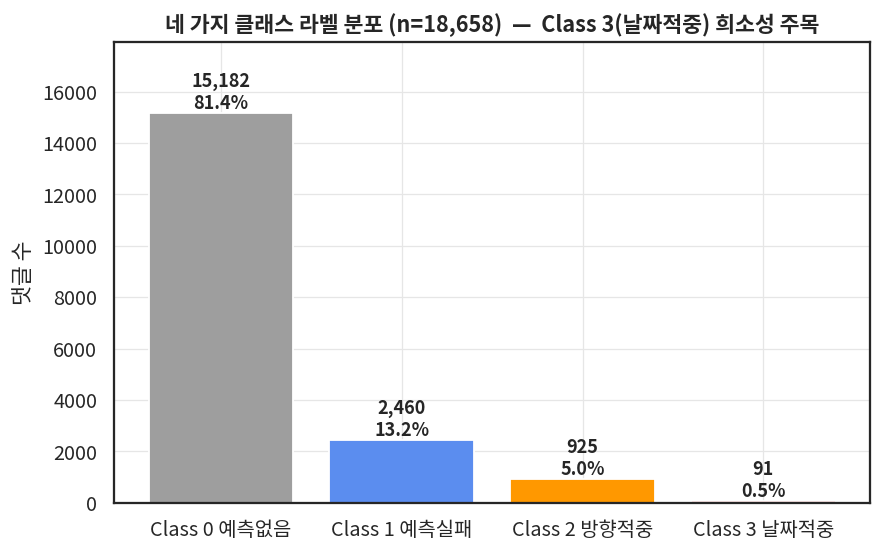
\includegraphics[width=\linewidth]{figures/fig6_class_dist.png}
\end{minipage}\hfill
\begin{minipage}{0.56\linewidth}\centering
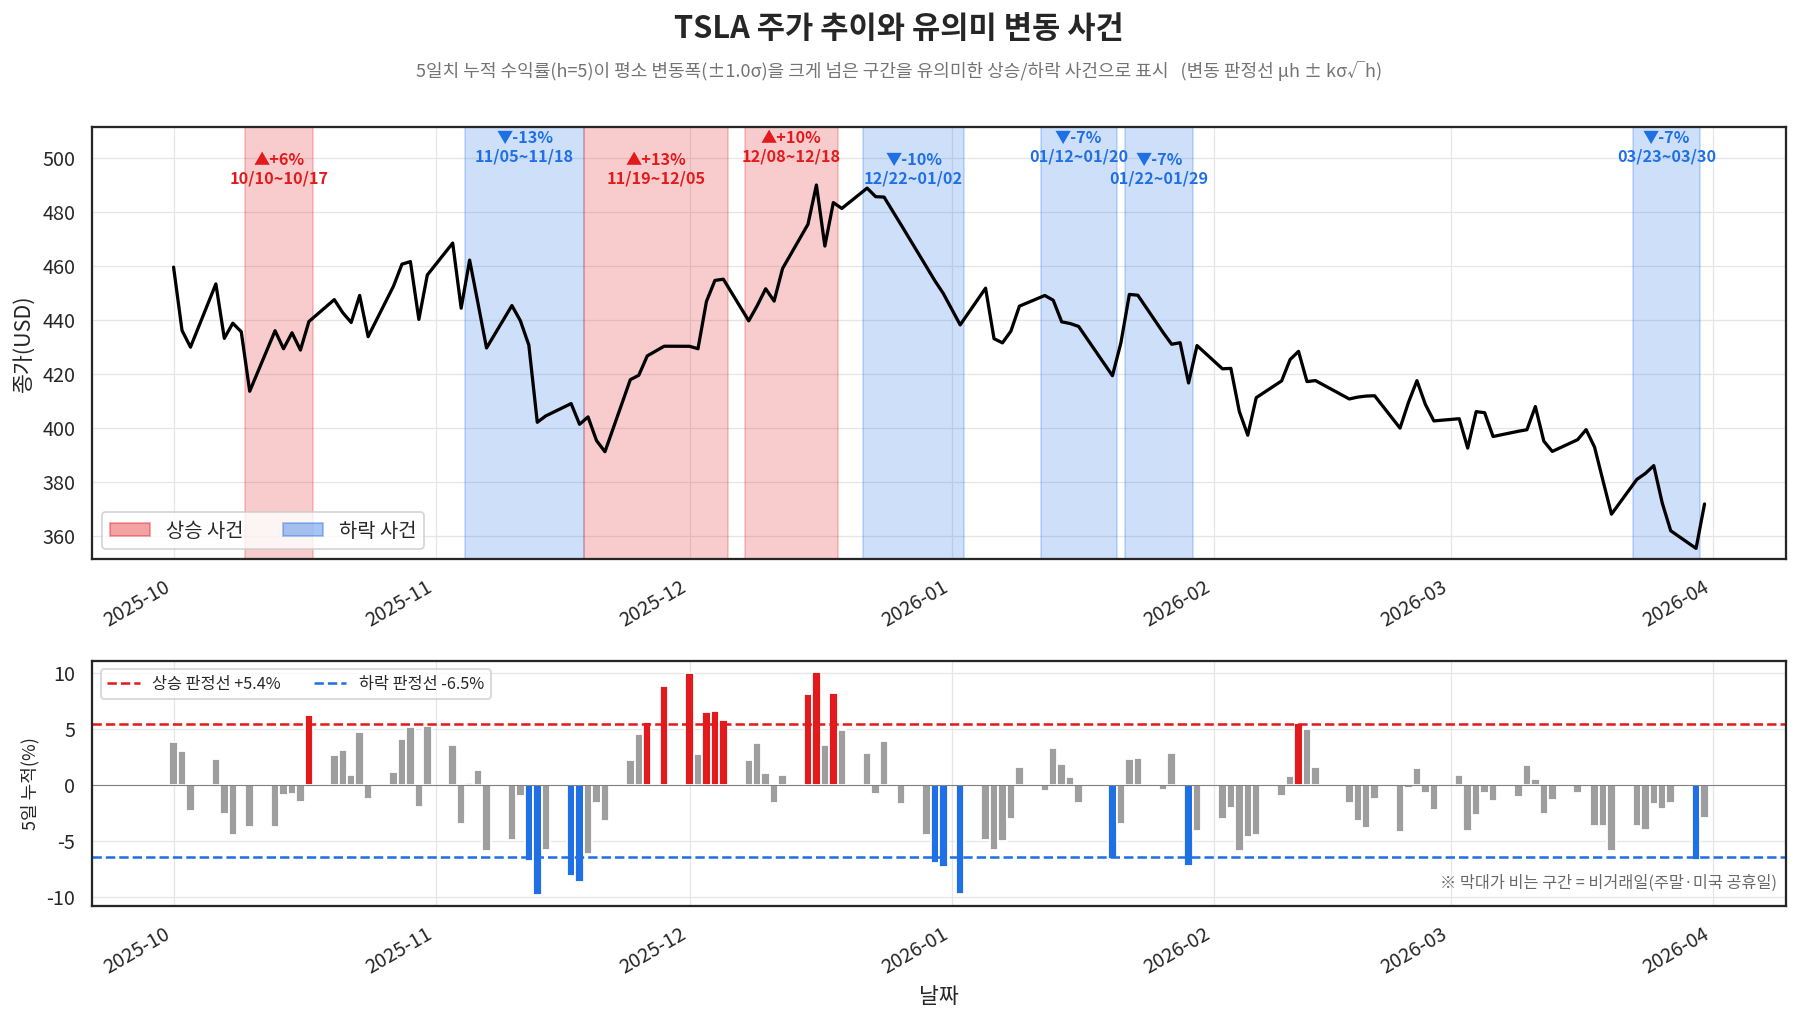
\includegraphics[width=\linewidth]{figures/fig1_price_story_TSLA.png}
\end{minipage}
\caption{탐색적 분석. 왼쪽은 클래스 분포로, 적중인 Class 2와 Class 3은 전체의 5.5\%, Class 3은 0.5\%에 불과하다. 오른쪽은 누적 기준 $h{=}5,\,k{=}1.0$으로 정의한 상승·하락 변동 사건 구간이며, 댓글이 그 주변에 집중된다. NVDA도 동일한 경향을 보이며 부록 B에 제시한다.}
\end{figure}

% ── 3. 모델 ─────────────────────────────────────────────────────────────────
\section{모델}

\subsection{모델 구조와 후보 모델}

모델 입력은 댓글 텍스트로 한정한다. 한국어 사전학습 인코더를 미세조정하는 구조를 사용하며, 문장 대표 벡터 \texttt{[CLS]}를 선형 분류 헤드에 연결하여 네 가지 클래스를 출력한다. 입력 텍스트 앞에는 \texttt{[주주]} 또는 \texttt{[비주주]} 토큰을 부착하고 임베딩 행렬을 확장하였으며, 뱃지 정보는 뱃지 보유를 실력자로 오인하는 잘못된 단서 학습을 방지하기 위하여 제외하였다.

도메인 특성이 상이한 세 한국어 인코더를 동일 조건에서 비교하였다. KcELECTRA는 댓글과 구어체, 신조어에 강건하여 주력 후보로 삼았고, KLUE-RoBERTa는 한국어 이해 과제의 표준 모델로서 비교 기준으로, KR-FinBERT는 금융 도메인 모델로서 대조군으로 선정하였다. 이는 정확도가 아니라 소수 클래스인 적중까지 잘 분류하는 모델을 선택하기 위함이다. 한편 KcELECTRA는 \texttt{[CLS]}와 \texttt{[SEP]} 토큰이 자동 부착되지 않는 문제가 있어 \texttt{TemplateProcessing}으로 보정하였다.

\subsection{기준 모델}

인코더의 실익을 가늠하기 위해 두 기준 모델과 비교한다. \textbf{다수 클래스} 기준선은 모든 입력을 최빈 클래스인 Class 0으로 예측하며, 불균형 데이터에서 정확도만 높고 소수 클래스는 전혀 맞히지 못하는 성능 하한을 제공한다. \textbf{TF-IDF + 로지스틱회귀} 기준선은 단어 빈도 기반의 선형 분류기로, 사전학습 표현 없이 표면적 어휘 단서만으로 도달할 수 있는 성능을 나타낸다. 인코더가 두 기준선을 얼마나 넘어서는지가 곧 문맥적 심층 표현이 적중 식별에 기여하는 정도이다. 모든 모델은 동일한 학습·평가 분할과 클래스 가중 손실 아래에서 비교하여, 성능 차이가 표현력에서 비롯되도록 통제하였다.

% ── 4. 실험 및 분석 ─────────────────────────────────────────────────────────
\section{실험 및 분석}

\subsection{손실함수 및 평가지표}

클래스 불균형이 심하므로, 표본 수가 적고 분류가 어려운 사례에 학습이 집중되도록 클래스 가중치와 focal 항을 결합한 손실을 사용하였다.
\begin{equation}
\mathcal{L}=\frac{1}{N}\sum_i (1-p_{t,i})^{\gamma}\cdot w_{y_i}\cdot\bigl(-\log p_{t,i}\bigr),\qquad
w_c=\sqrt{N/(C\cdot n_c)},\ \ \gamma=2
\end{equation}
주 평가지표로는 소수 클래스를 동등하게 반영하는 macro-F1, 곧 클래스별 F1의 산술 평균을 채택하였으며, 모델 선택과 early stopping의 기준에도 동일하게 적용하였다. 정확도는 보조 지표로만 활용하였다.

\subsection{데이터 분할 및 학습 방법}

다른 종목에 대한 일반화를 검증하기 위해 종목을 분리하여 TSLA로 학습하고 NVDA로 평가하였다. early stopping과 모델 선택에 사용하는 검증셋은 학습셋 내부에서 15\%를 분리하여 테스트셋과 격리하였고, 학습에 등장한 작성자는 테스트셋에서 제거함으로써 특정 작성자의 문체 암기를 방지하였다. 데이터 구성은 표 2와 같다.

\begin{table}[H]
\centering
\begin{tabular}{@{}llll@{}}
\toprule
\textbf{구분} & \textbf{종목} & \textbf{규모} & \textbf{용도} \\
\midrule
훈련 & TSLA & 보강 후 28,038건, 적중 969건 & 모델 파라미터 학습 \\
검증 & TSLA & 훈련셋의 15\%, 약 4,200건 & early stopping 및 모델 선택 \\
테스트 & NVDA & 자연 분포 3,667건 & 다른 종목에 대한 일반화 평가 \\
\bottomrule
\end{tabular}
\caption{훈련·검증·테스트 구성. 테스트는 종목을 달리하여 일반화를 평가한다.}
\end{table}

학습은 두 단계로 수행하였다. 1단계에서는 2.2절의 라벨, 곧 \emph{1차 라벨}로 기본 모델을 학습하여 적중 식별 신호의 유무를 확인한다. 그런데 적중(Class 2·3) 표본이 매우 적어 학습이 어려우므로, 2단계에서는 적중 표본을 늘리는 \emph{2차 라벨링}을 수행한다. 구체적으로 1차에서 적중이 잦았던 고수 후보와 무작위 대조군을 추린 뒤 이들의 추가 댓글을 다시 라벨링하였고, 이로써 적중 댓글이 643건에서 969건으로, Class 2는 608에서 909건, Class 3은 35에서 60건으로 늘었다. 이렇게 보강한 학습셋으로 재학습한 것이 2단계이며, 보강은 댓글 단위로만 수행하였다. 2차 표본 구성의 자세한 내용은 부록 C에 정리하였다. 표 2의 훈련 규모는 보강 학습셋 기준이고, 주요 하이퍼파라미터는 표 3과 같다. 하이퍼파라미터는 세 인코더에 동일하게 적용하여 모델 간 비교를 공정하게 하였고, 모델별 개별 탐색 대신 클래스 가중 focal 손실과 macro-F1 기준 조기 종료로 불균형에 대응하였다.

\begin{table}[H]
\centering
\begin{tabular}{@{}llll@{}}
\toprule
\textbf{항목} & \textbf{값} & \textbf{항목} & \textbf{값} \\
\midrule
Encoder & 한국어 사전학습 인코더 & Optimizer & AdamW (fp16) \\
Epochs & 6 & Early stopping & patience 3 \\
Batch size & 32 & Learning rate & $1\!\times\!10^{-5}$ \\
Max length & 512 (dynamic padding) & Warmup ratio & 0.1 \\
Loss & class-weighted focal ($\gamma{=}2$) & Weight decay & 0.01 \\
Seed & 42 & Baseline & 다수 클래스 · TF-IDF \\
\bottomrule
\end{tabular}
\caption{주요 학습 설정. 세 인코더와 두 단계에 동일한 seed와 데이터 분할로 적용하였다.}
\end{table}

\subsection{분류 결과}

테스트셋은 NVDA 자연 분포로 표본 수는 $n{=}3{,}667$이며, 클래스별로는 Class 0이 3,153건, Class 1이 141건, Class 2가 317건, Class 3이 56건이다. 교차 평가 결과는 표 4 및 표 5와 같다.

\begin{table}[H]
\centering
\begin{tabular}{@{}lcccccc@{}}
\toprule
\textbf{모델 / 기준선} & \textbf{macro-F1} & \textbf{정확도} & \textbf{Class 0} & \textbf{Class 1} & \textbf{Class 2} & \textbf{Class 3} \\
\midrule
KLUE-RoBERTa            & \textbf{0.389} & 0.810 & 0.925 & 0.217 & 0.184 & 0.232 \\
KR-FinBERT              & 0.343 & 0.802 & 0.920 & 0.211 & 0.175 & 0.069 \\
KcELECTRA               & 0.342 & 0.813 & 0.930 & 0.223 & 0.214 & 0.000 \\
\addlinespace[1pt]\midrule\addlinespace[1pt]
기준선 TF-IDF + 로지스틱회귀 & 0.323 & 0.757 & 0.882 & 0.123 & 0.116 & 0.170 \\
기준선 다수 클래스          & 0.231 & 0.860 & 0.925 & 0.000 & 0.000 & 0.000 \\
\bottomrule
\end{tabular}
\caption{1단계 원본 라벨 학습의 교차 평가. TSLA로 학습한 뒤 NVDA로 평가하였으며, Class 0부터 Class 3 칸은 클래스별 F1이다.}
\end{table}

\begin{table}[H]
\centering
\begin{tabular}{@{}lcccccc@{}}
\toprule
\textbf{모델} & \textbf{macro-F1} & \textbf{정확도} & \textbf{Class 0} & \textbf{Class 1} & \textbf{Class 2} & \textbf{Class 3} \\
\midrule
KLUE-RoBERTa & \textbf{0.350} & 0.825 & 0.934 & 0.232 & 0.107 & 0.127 \\
KR-FinBERT   & 0.349 & 0.819 & 0.930 & 0.239 & 0.156 & 0.069 \\
KcELECTRA    & 0.329 & 0.820 & 0.935 & 0.231 & 0.148 & 0.000 \\
\bottomrule
\end{tabular}
\caption{2단계 보강 학습셋 재학습의 교차 평가. 테스트셋은 동일한 자연 분포이며 숫자는 클래스별 F1이다.}
\end{table}

\begin{figure}[H]
\centering
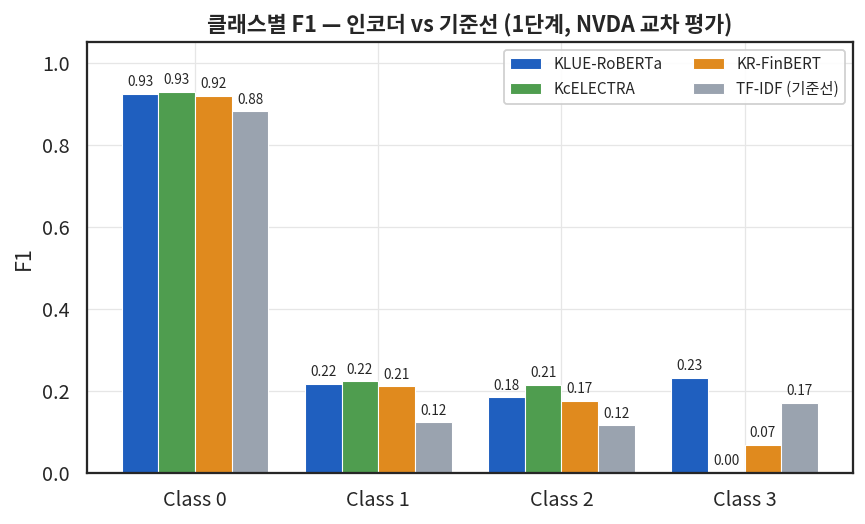
\includegraphics[width=0.54\linewidth]{figures/fig_perclass_f1.png}
\caption{클래스별 F1 비교(1단계, NVDA 교차 평가). 다수 클래스인 Class 0은 0.9 안팎이나 적중인 Class 2·3은 0.0--0.23에 머물며, 인코더는 대체로 TF-IDF 기준선을 웃돈다.}
\end{figure}

\textbf{식별 신호의 존재.} 그림 2는 표 4의 클래스별 F1을 인코더와 기준선에 대해 비교한 것이다. 세 인코더는 모두 다수 클래스 0.231과 TF-IDF 0.323 기준선을 웃돌아, 텍스트만으로도 적중 댓글을 기준선 이상으로 가려내는 약하지만 분명한 신호가 있음을 보여준다.

\textbf{소수 클래스의 한계.} 그러나 그림 2에서 드러나듯 다수 클래스인 Class 0의 F1은 0.93 수준으로 높은 반면, 적중에 해당하는 Class 2와 Class 3의 F1은 0.0에서 0.23 사이에 머문다. 오류 분석 결과 방향 적중인 Class 2는 대부분 실패인 Class 1로 오분류되었다. 이는 텍스트만으로 적중과 실패를 구분하기가 근본적으로 어려움을 의미한다. 작성자 단위에서 적중이 지속되는지는 4.4절에서 살펴본다.

\textbf{보강의 한계.} 표본 보강 이후에도 최고 macro-F1은 0.389에서 0.350으로 오히려 하락하였으며, 특히 Class 3의 F1은 0.232에서 0.127로 감소하였다. 학습용 Class 3 표본이 60건에 불과하여 보강만으로는 희소성이 해소되지 않았기 때문이다. 다만 1단계에서 학습 데이터를 늘릴수록 Class 2의 F1이 0에서 0.024, 0.048, 0.065로 꾸준히 상승한 점은 신호의 부재가 아니라 표본 부족이 원인임을 시사한다.

\subsection{추가 분석: 작성자 단위 적중의 지속성}

적중이 작성자의 지속적 특성인지 확인하기 위해, 적중이 잦은 작성자를 전·후반으로 나누어 초과 적중률을 비교하였다. 두 기간의 초과 적중률 사이에는 상관이 거의 없어 상관계수가 0.07에 그쳤다(그림 3). 즉 한때 잘 맞힌 작성자가 이후에도 잘 맞히지는 않았다.

이는 적중·고수 후보 표본이 고변동 구간에서 활발히 활동한 사용자, 곧 단기 매매 성향에 편중되어 추출된 데 따른 것으로 보인다. 변동이 본격화되기 이전에 예측하는 중장기 관점의 예측자는 거의 포착되지 못하였으며, 이들을 추가로 관찰하면 적중 클래스(Class 2·3)의 불균형이 완화될 가능성이 있다. 이는 후속 연구로 남긴다.

\begin{figure}[H]
\centering
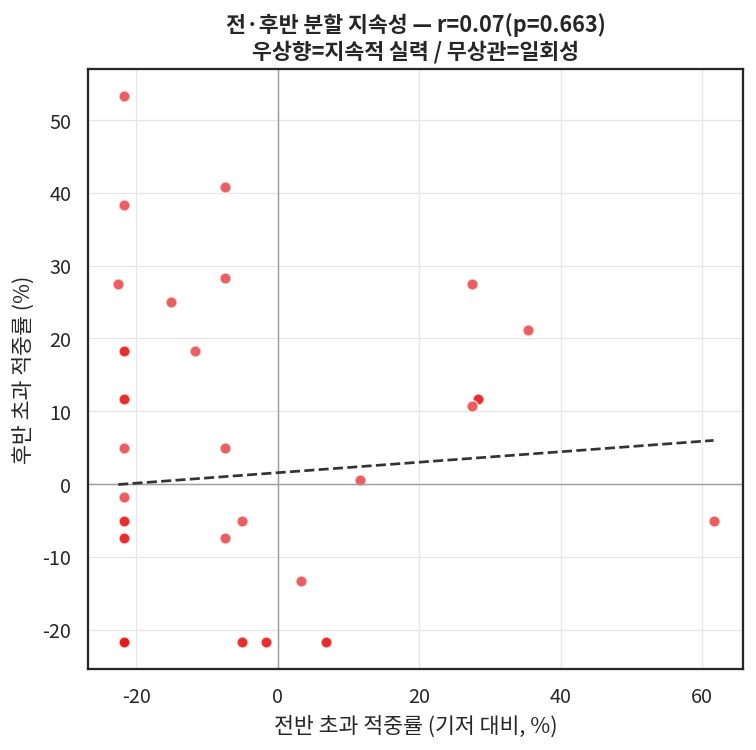
\includegraphics[width=0.5\linewidth]{figures/fig12_split_half.png}
\caption{적중이 잦은 작성자의 전·후반 초과 적중률. 상관이 거의 없어(상관계수 0.07) 작성자 단위로도 적중이 꾸준히 지속되지는 않는다.}
\end{figure}

% ── 5. 결론 ─────────────────────────────────────────────────────────────────
\section{결론}

\textbf{결과 요약.} 댓글 텍스트만으로 적중 예측을 식별하는 분류기는 세 인코더 모두에서 다수 클래스와 TF-IDF 기준선을 웃돌았다. 텍스트만으로도 적중 댓글을 가려내는 약하지만 분명한 신호가 있다는 뜻이다. 다만 적중에 해당하는 소수 클래스의 성능은 낮았으며, 적중 신호는 단일 댓글에 약하고 작성자 단위로도 안정적이지 않았다. 학습 곡선이 표본 증가에 따라 꾸준히 상승한 점은 이러한 한계가 신호의 부재가 아니라 적중 표본의 희소성에서 비롯됨을 시사한다.

\textbf{한계.} 첫째, 테스트셋인 NVDA가 상승장이어서 하락 적중 사례가 전무하였고, 이로 인해 실제 적중 식별과 상승장에서의 강세론적 문체를 분리하여 검증하지 못하였다. 둘째, 적중 특히 Class 3 표본의 절대량이 부족하여(학습용 60건) 소수 클래스 학습이 제약된다. 셋째, 작성자 단위 분석의 표본이 41명으로 작아 검정력이 낮다. 넷째, 라벨은 사람 검수를 거치지 않은 자동 생성 라벨이며, 고용량 모델 사용으로 신뢰도를 보완하였으나 검수 기반 라벨로의 확장은 후속 과제로 남는다.

\textbf{향후 개선 방향.} NVDA로 학습하고 TSLA로 평가하는 반대 방향은 하락 표본을 보유하므로 이를 통해 하락 적중을 검증하고, 적중 표본을 확충하여 학습 곡선의 포화 지점을 확인하며, 적중과 실패를 더 잘 분리하도록 능동 학습이나 어려운 표본 가중을 적용하고자 한다.

% ── 부록 ────────────────────────────────────────────────────────────────────
\clearpage
\section*{부록}
\addcontentsline{toc}{section}{부록}
{\small 본 절은 본문 이해에 필수적이지는 않은 보조 분석 및 그림을 정리한 것이다.}

\subsection*{A. 데이터 추출 구간}

1차와 2차는 추출 방식이 다르다. \textbf{1차}는 고변동 \emph{구간} 단위로, 변동 사건 주변 구간(그림 4 위의 녹색 박스) 안의 댓글을 모아 훈련(TSLA)·평가(NVDA) 세트를 구성하였다. \textbf{2차}는 \emph{사용자} 단위로, 1차 구간에 나타난 작성자 가운데 적중이 잦은 고수 후보 130명과 무작위 대조군 130명을 1 대 1로 뽑은 뒤, 이 사용자들의 댓글을 6개월 전 구간에 걸쳐 추가로 라벨링하였다(그림 4 아래). 음영은 상승·하락 변동 사건이다.

\begin{figure}[H]
\centering
\begin{minipage}{0.43\linewidth}\centering

\includegraphics[width=\linewidth]{figures/tsla_train.png}\\[2pt]

\includegraphics[width=\linewidth]{figures/expert_control_tsla.png}
\end{minipage}\hfill
\begin{minipage}{0.43\linewidth}\centering

\includegraphics[width=\linewidth]{figures/nvda_eval.png}\\[2pt]
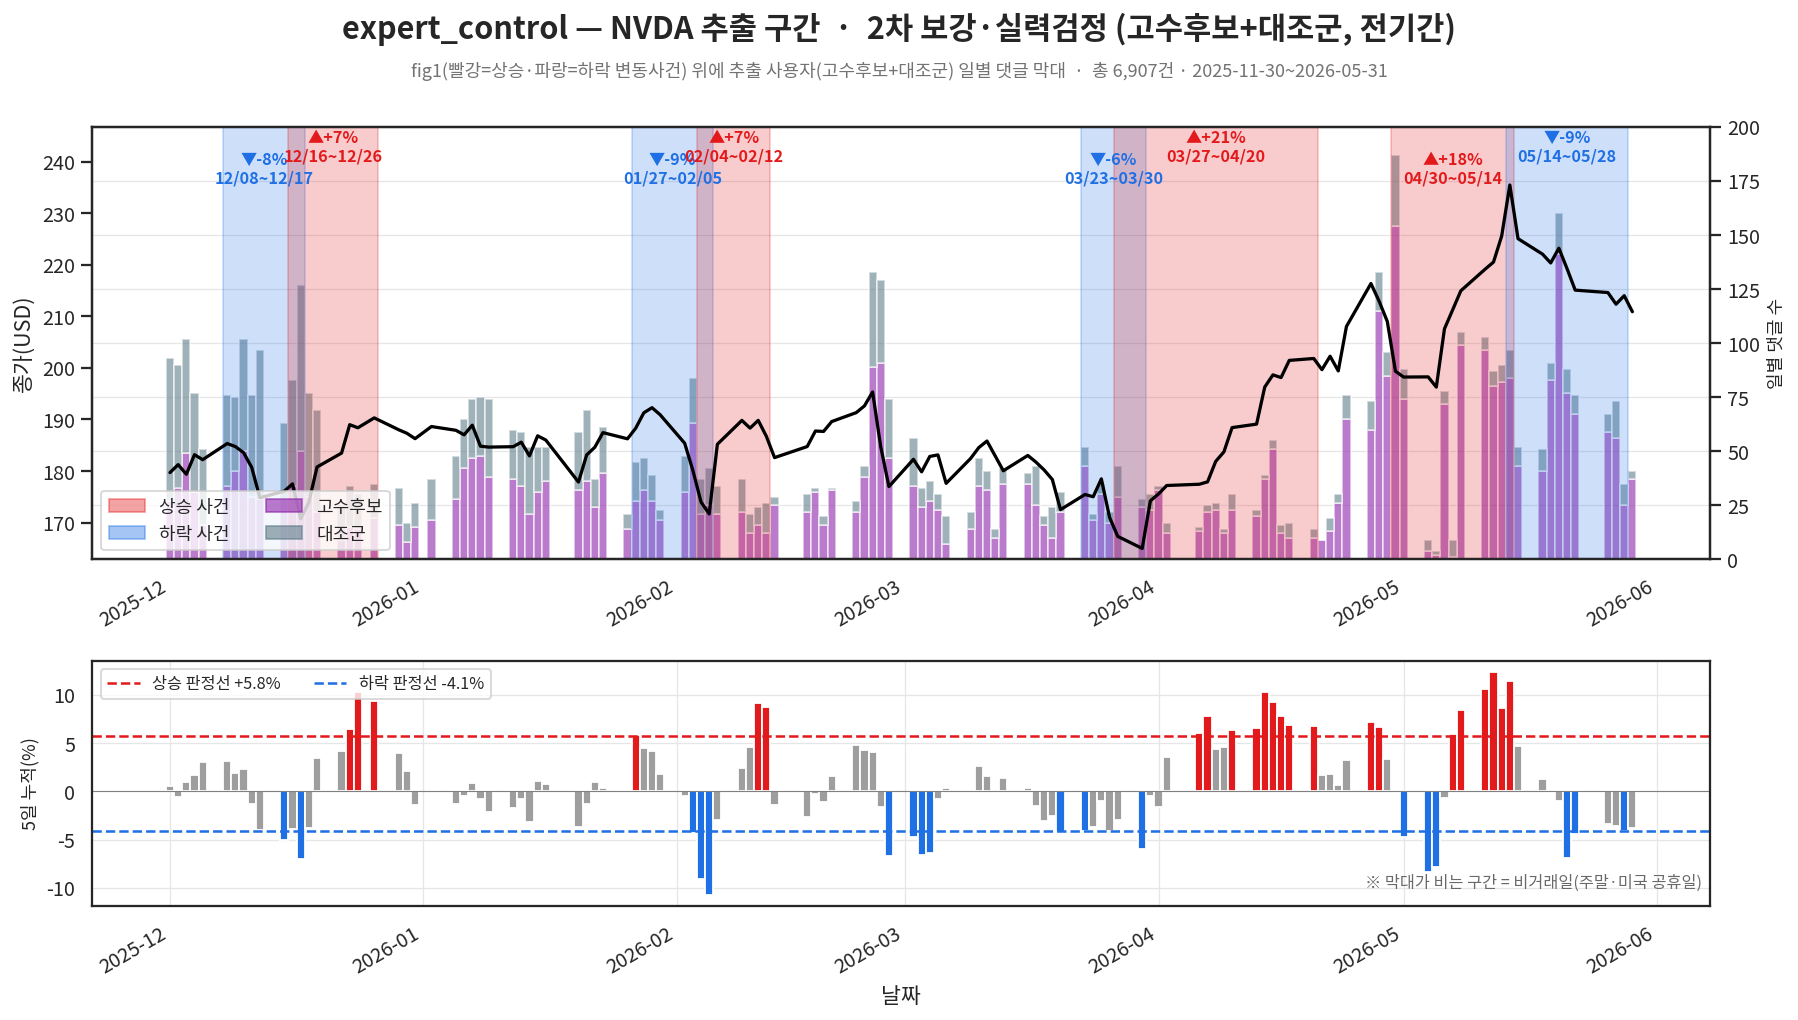
\includegraphics[width=\linewidth]{figures/expert_control_nvda.png}
\end{minipage}
\caption{부록 A. 데이터 추출 구간. 위는 1차의 구간 단위 추출(녹색 박스)로 만든 훈련(TSLA)·평가(NVDA) 세트, 아래는 2차에서 선정한 고수 후보·대조군 사용자의 6개월 전 구간 일별 활동이다.}
\end{figure}

\subsection*{B. 변동 사건 정의와 판정 기준값}

변동 사건은 누적 $h$거래일 수익률이 판정선 $\mu_h \pm k\,\sigma\sqrt{h}$를 벗어나는 구간으로 정의한다. 여기서 $h$는 누적 기간, $k$는 판정폭 계수이며, $k$를 키우면 더 큰 변동만 사건으로 인정되어 사건 수가 줄어든다. 본문 그림 1의 NVDA 판본은 그림 5 왼쪽으로, 두 종목 모두 댓글이 변동 사건 주변에 집중된다.

기준값 $h$와 $k$는 그림 5 오른쪽의 탐색으로 정하였다. 두 지표를 함께 보았는데, \emph{변동 지속율}(사건 이후에도 변동이 이어지는 비율로, 높을수록 일시적 잡음이 아닌 진짜 사건)과 유의미한 변동 사건의 비율·수이다. $k{=}1.5$로 키우면 판정폭이 넓어져 유의미한 변동 사건이 과도하게 줄어들므로 $k{=}1.0$으로 두었고, $k{=}1.0$에서 변동 지속율이 높으면서 사건 수도 충분한 $h{=}5$를 택하였다.

\begin{figure}[H]
\centering
\begin{minipage}{0.46\linewidth}\centering
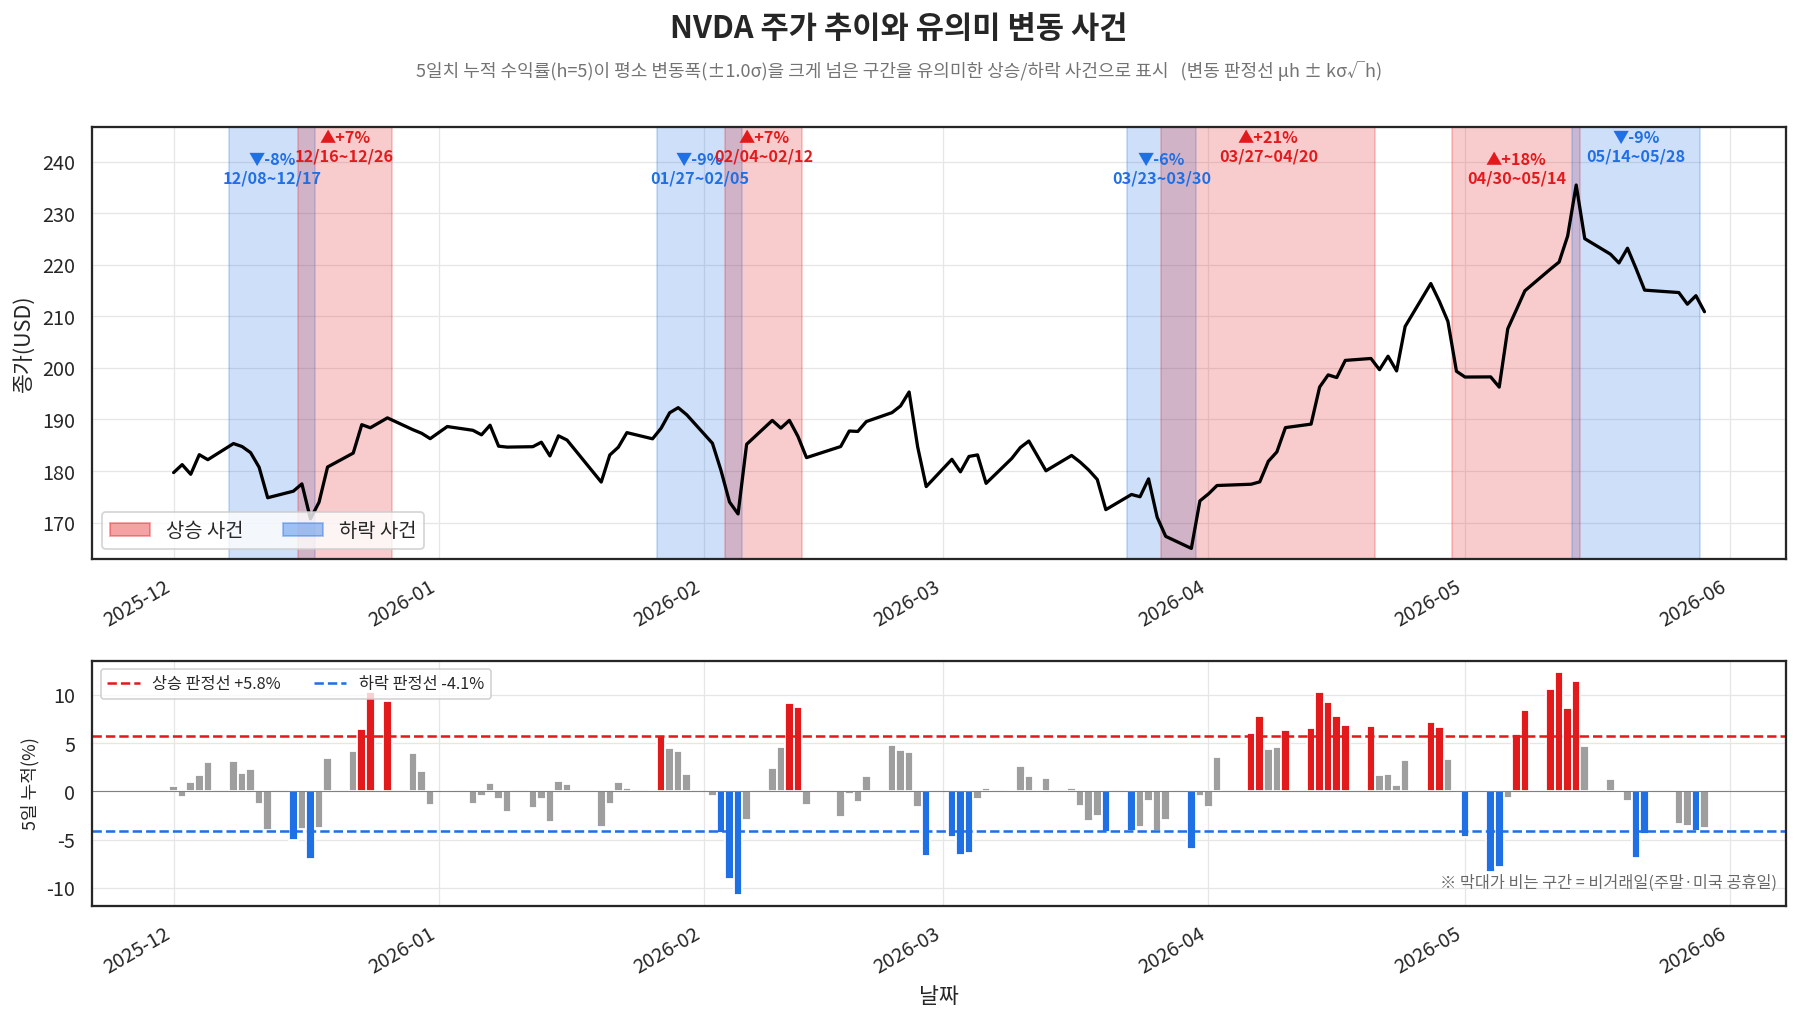
\includegraphics[width=\linewidth]{figures/fig1_price_story_NVDA.png}
\end{minipage}\hfill
\begin{minipage}{0.52\linewidth}\centering
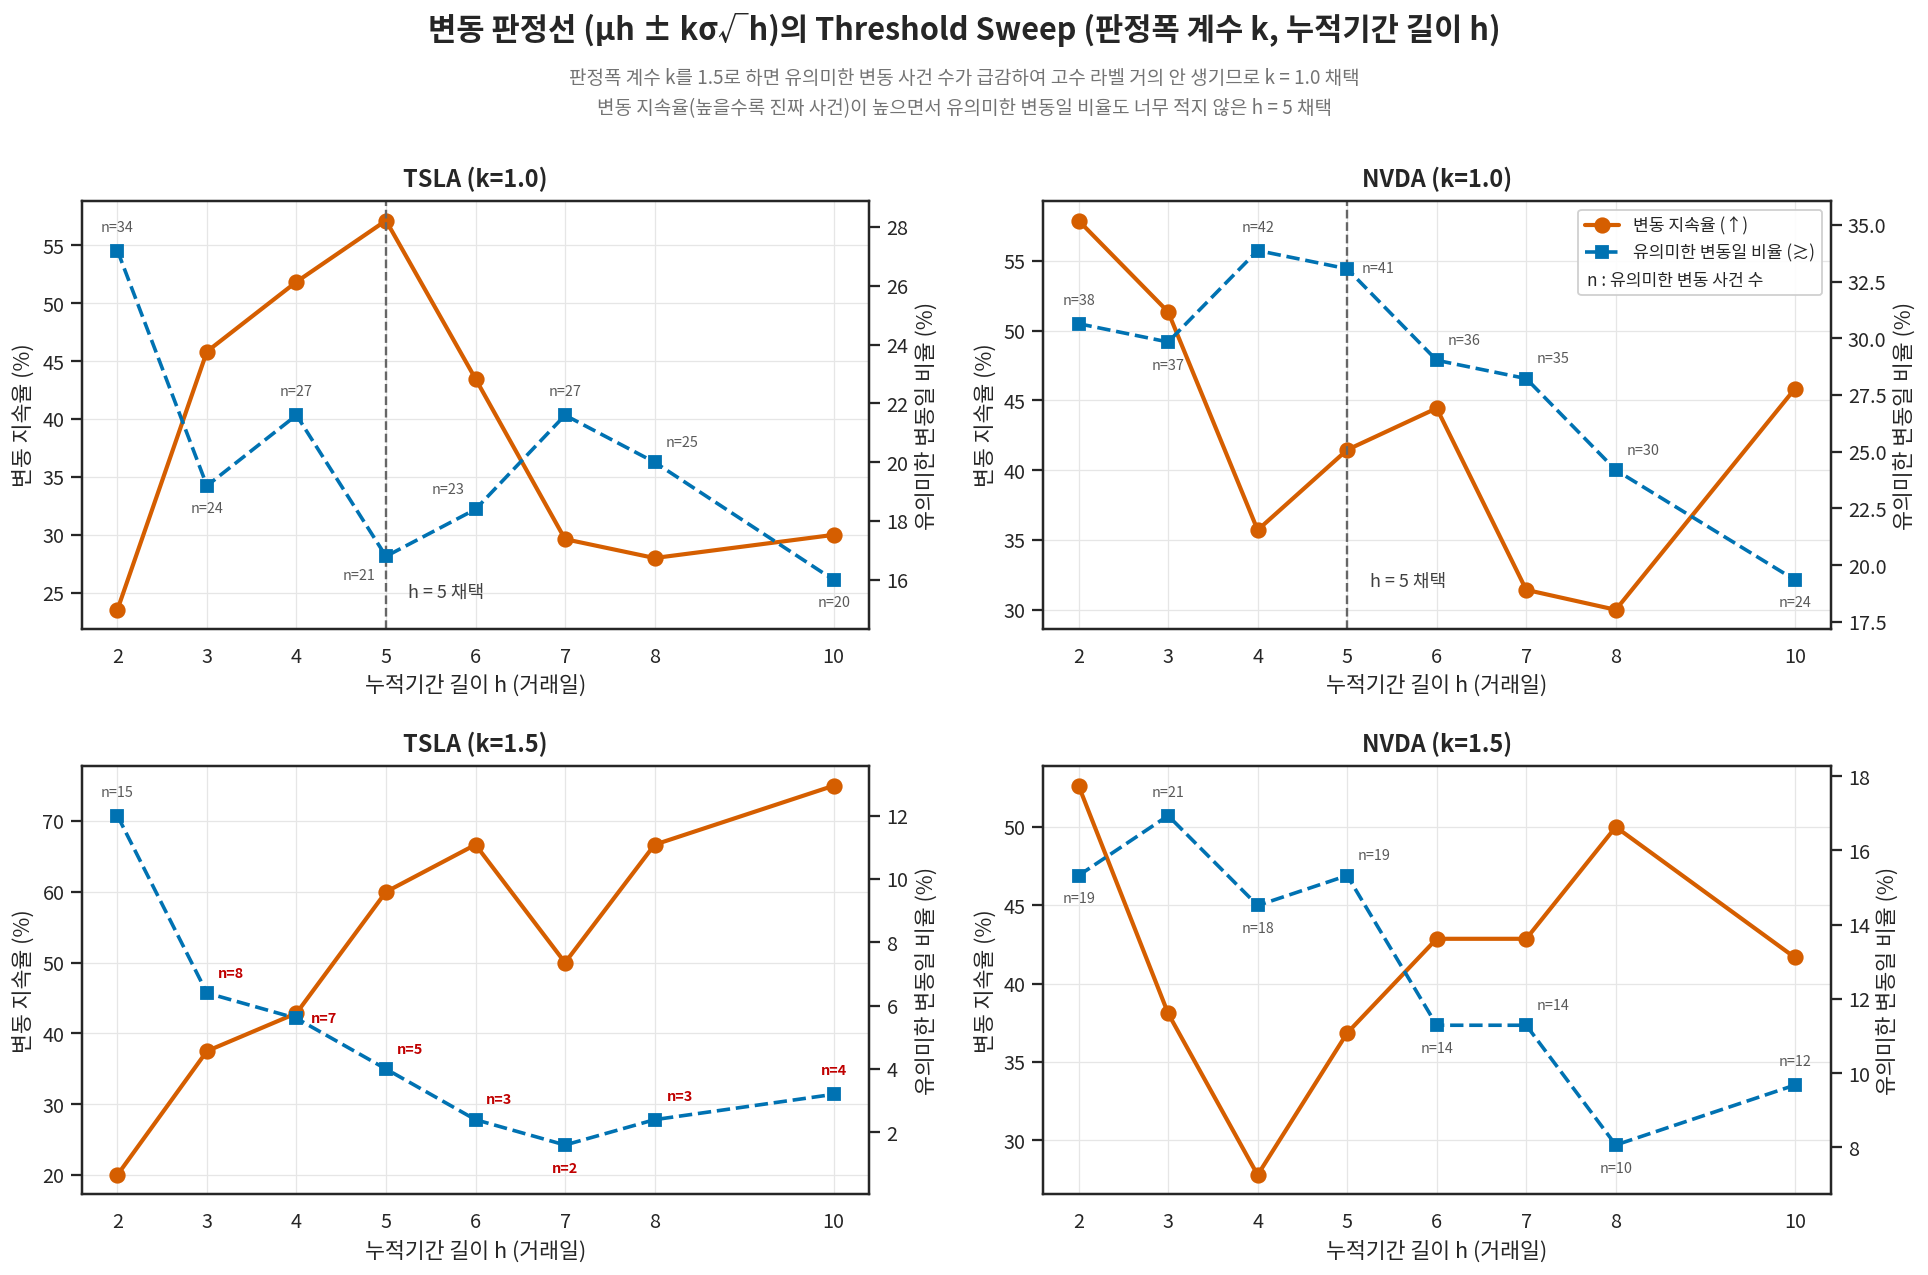
\includegraphics[width=\linewidth]{figures/fig2_threshold_sweep.png}
\end{minipage}
\caption{부록 B. 왼쪽은 NVDA 주가 추이와 변동 사건이고, 오른쪽은 변동 판정 기준값 $h$와 $k$의 탐색 결과이다.}
\end{figure}

\subsection*{C. 2차 라벨링 표본 구성과 작성자 단위 분석}

2차 라벨링 표본은 1차 라벨을 기준으로 구성하였다. 1차에서 적중(Class 2·3)이 2건 이상인 작성자를 \emph{고수 후보}(130명)로, 예측은 하였으나 적중이 거의 없던 작성자 중 무작위로 같은 수를 \emph{대조군}(130명)으로 선정한 뒤, 이들의 추가 댓글을 다시 라벨링하여 적중 표본을 보강하였다(본문 4.2).

선정된 두 집단이 실제로 실력 차이를 보이는지 점검하였다. 작성자별 적중률의 과분산 검정에서는 분산비 1.71($p<.001$)로 일부 작성자에 적중이 쏠리는 듯 보였다. 그러나 2차 실력 점수 상위 10명 가운데 5명이 대조군이어서 사전에 고른 고수 후보가 더 낫지 않았고(그림 6, 두 집단 차이 $p=0.665$), 본문 4.4의 전·후반 지속성에서도 그 쏠림은 유지되지 않았다. 따라서 작성자 단위 보강은 특정 작성자의 문체 암기와 테스트셋 누수 위험만 키우므로 댓글 단위 보강만 채택하였다.

\begin{figure}[H]
\centering

\includegraphics[width=0.78\linewidth]{figures/skill_top10.png}
\caption{부록 C. 2차 실력 점수 상위 10명. 고수 후보와 대조군이 5 대 5로 혼재하여 사전 선정 집단의 우위가 관찰되지 않는다.}
\end{figure}

\end{document}
